\documentclass[conference]{IEEEtran}

\usepackage{amssymb}
\usepackage{amsmath}
\usepackage{array}
\usepackage{booktabs}
\usepackage{graphicx}
\usepackage[hidelinks]{hyperref}
\usepackage{siunitx}
\usepackage[final]{microtype}

\emergencystretch=2em
\raggedbottom

\providecommand{\papergraphicsroot}{./}
\providecommand{\paperbibfile}{references}
\graphicspath{{\papergraphicsroot}{paper/}}

\newcommand{\btc}{Bitcoin}
\newcommand{\datafile}[1]{\nolinkurl{#1}}
\newcolumntype{L}[1]{>{\raggedright\arraybackslash}p{#1}}

\begin{document}

\title{Store of Value, Not Daily Payment:\\
Evidence from \btc{} Transaction Data}

\author{\IEEEauthorblockN{Junhyuk Lee}
\IEEEauthorblockA{Department of Computer Science and Engineering\\
Texas A\&M University\\
College Station, TX, USA\\
xodn348@tamu.edu}
\and
\IEEEauthorblockN{Korok Ray}
\IEEEauthorblockA{James Benjamin Department of Accounting\\
Mays Business School, Texas A\&M University\\
College Station, TX, USA\\
korok@mays.tamu.edu}}

\maketitle

\begin{abstract}
Did \btc{}'s on-chain use shift from a medium-of-exchange role toward
a store-of-value role between 2021 and 2026? We answer this question using
on-chain transaction data, combining current UTXOs, full-node block
transactions, and address-level balances rather than relying on price data.
At height 950{,}696, the chainstate snapshot shows that 60.5\% of current
BTC has not moved on chain for at least one year, and 33.3\% has not moved
for at least five years. The full-node block analysis adds an activity
measure. Most transaction output sums are small, but the upper tail remains
settlement-sized across the five-year window. The address parser maps
19.92 million BTC to 56.05 million addresses and shows that balances are
concentrated rather than distributed like daily-use balances. Taken
together, these measurements reject the simplest daily-payment
interpretation. Bitcoin still supports on-chain payments, but the observed
transaction data are more consistent with savings, custody, large transfers,
and operational consolidation. The on-chain record for 2021 to 2026 is
therefore more consistent with store-of-value and settlement infrastructure than with
a daily payment rail.
\end{abstract}

\begin{IEEEkeywords}
Bitcoin, transaction data analysis, address analysis, store of value
\end{IEEEkeywords}

\section{The Question}\label{sec:intro}

This paper asks whether \btc{}'s on-chain use shifted toward a
store-of-value role rather than a medium-of-exchange role between 2021 and
2026
\cite{nakamoto2008bitcoin, yermack2015bitcoin, liu2021risks,
makarov2020trading}. The distinction matters because Bitcoin transactions
can support retail payment, settlement, custody, treasury management,
speculation, and long-term saving. Price data alone
cannot show which use is most visible on chain. We therefore measure the
transaction data directly. The macro and block-flow evidence covers
2021 to 2026, and the on-chain analysis uses live UTXOs, full-node block
transactions, and current-output address balances derived from Bitcoin Core.

This period is informative because several major events were concentrated
within it, including the 2021 risk peak, the rate-hiking cycle from 2022 to
2023, the FTX-related trust shock, US spot exchange traded fund approval, the
fourth halving, Mt.\,Gox creditor distributions, and Taproot-related protocol
changes. These events changed the cost of holding risky assets, the trust
placed in custodians, and the availability of regulated access. If \btc{}
became more consistent with savings and settlement infrastructure, that
shift should be visible in three places. The first is the share of coins
that remain unspent. The second is the size distribution of transactions
that do move. The third is the address structure of current balances.

The evidence is more consistent with store-of-value use than with daily
payment use. Many current BTC have not moved for at least one, three, or
five years. When coins do move, most transaction output sums are small, but
the largest transactions remain very large. At the address level, BTC
balances and UTXO counts are concentrated even without wallet or entity
clustering. Taken together, the stock, flow, dormancy, and address evidence
support the store-of-value interpretation.

This paper does not attempt to deanonymize users. Prior work already showed
that address graphs, multi-input heuristics, and clustering can reveal
important structure in cryptocurrency systems
\cite{meiklejohn2013fistful, reid2013analysis, androulaki2013evaluating,
harrigan2016unreasonable, goldfeder2018cookie}. The goal here is narrower.
We use Bitcoin Core data to identify what the transaction record itself
shows. We keep the unit of observation explicit and separate direct on-chain
evidence from claims about owners, wallets, or motives that the data cannot
identify.

\section{Related Measurement Work and Identification}\label{sec:related}

Two measurement issues matter for this paper. First, the blockchain records
transactions exactly, but it does not record intent. A full node can tell
whether an output is unspent, when it was created, which script family
controls it, and which transactions appear in the full-node block window.
Those facts do not reveal whether a user intended to save, trade, pay,
consolidate, or rotate a vault. Address clustering and entity attribution
can add useful context, but they also add assumptions that can fail when
wallets change behavior or custodians aggregate users
\cite{meiklejohn2013fistful, moser2017anonymous, kalodner2020blocksci,
moser2022resurrecting}.

Second, payments and savings are measured with different units. Payment use
is a flow concept, measured by how often coins move, how large transfers
are, and whether outputs are quickly spent. Store-of-value use is a stock
concept, measured by how much BTC remains unspent, how old the live outputs
are, and how concentrated the live balances are. A transaction sample describes what
happens when coins move. A UTXO snapshot describes what remains spendable
and unspent at a point in time. Address-level aggregation describes how that
current stock is distributed across script-derived address strings, not
across economic owners.

The approach is deliberately cautious
\cite{manski1990nonparametric, manski2003partial}. We do not label wallets,
exchanges, merchants, or lost coins. Instead, we ask what Bitcoin Core data
show when the interpretation is kept narrow. A single statistic could be
misleading. A large old UTXO stock, a large-transaction tail, and
concentrated current address balances are different measurements. Their
agreement is therefore more informative than any single measure.

\section{Macroeconomic and Protocol Setting}\label{sec:setting}

The setting matters because Bitcoin transactions can serve different uses
under different market conditions. From 2021 to 2026, \btc{} passed through
a rate-hiking cycle, the FTX-related trust shock, regulated ETF access, the
fourth halving, and wider use of Taproot-related custody tools.
Figure~\ref{fig:macro-timeline} places those events on one timeline. The
shaded bands mark broad market regimes; the upper row marks macro,
regulatory, and custody events; and the lower row marks protocol and
blockspace events.

\begin{figure*}[!tbp]
  \centering
  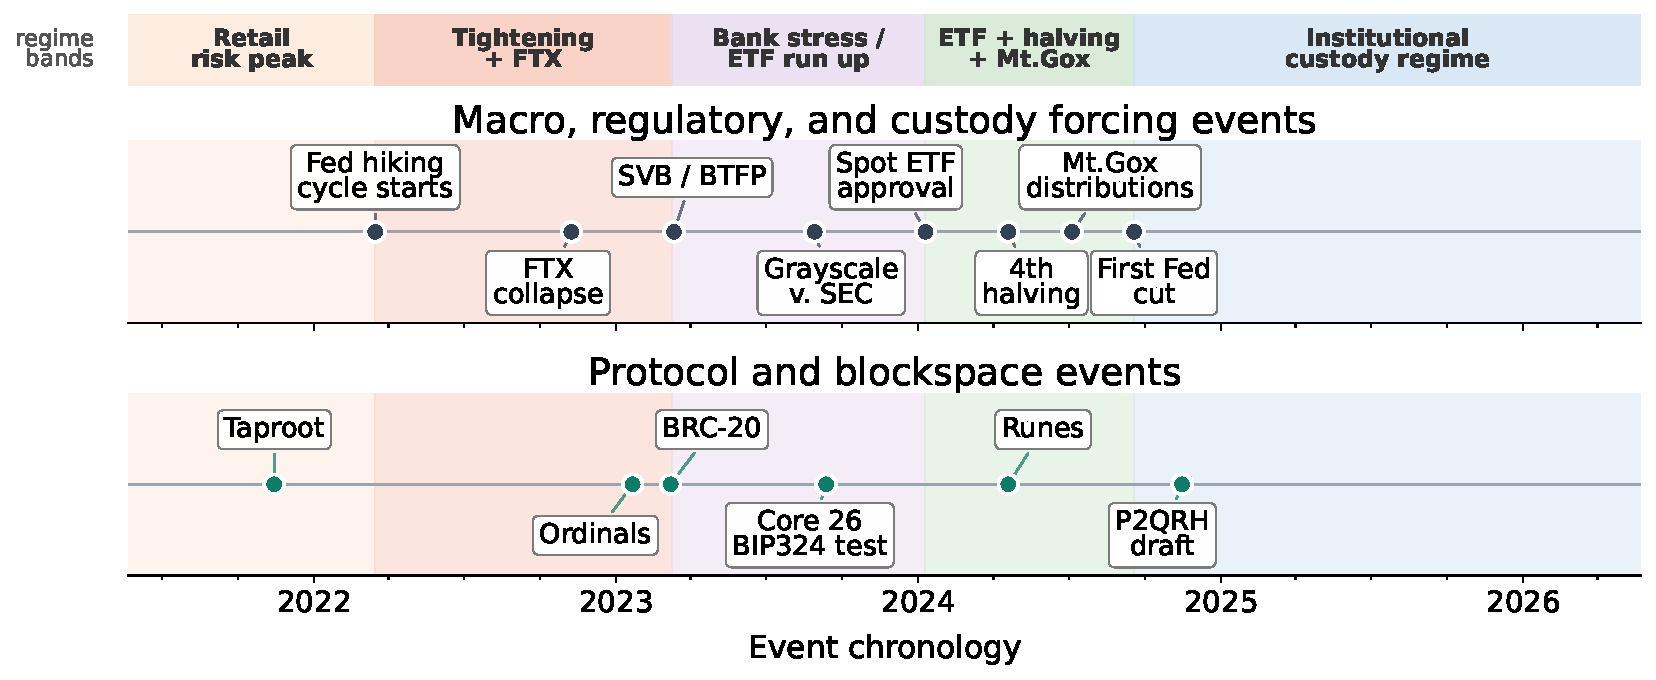
\includegraphics[width=0.94\textwidth]{figures/fig01_macro_protocol_timeline.pdf}
  \caption{Macroeconomic and protocol timeline, 2021 to 2026. Shaded bands
  mark market regimes; upper markers show macro, regulatory, and custody
  events; lower markers show protocol and blockspace events.}
  \label{fig:macro-timeline}
\end{figure*}

The economic background also changed who could hold BTC and how they could
hold it. The sample begins near the 2021 retail risk peak, when \btc{}
traded with other speculative assets. Tightening then made that trade more
expensive. From March~2022 to July~2023 the Federal Reserve raised rates by
525 basis points, and the FTX collapse increased perceived exchange-custody
risk. In 2023, regional-bank stress made self-custody and scarce collateral
more important, while the Ripple and Grayscale decisions made regulated
market access more realistic. By January~2024, spot ETF approval shifted
access from mostly direct exchange accounts to regulated brokerage and
custody channels. The halving, the start of Mt.\,Gox distributions, the
first Fed cut, and the 2025 CLARITY Act process all arrived after that
access point. The timing matters because the market no longer had to rely only on retail
trading demand to absorb supply \cite{ftxbankruptcy2022,
secripple2023, grayscalesec2023, sec2024etfapproval, mtgoxtrustee2024}.

The technical environment also changed. Bitcoin's monetary rule did not
change, but tools for large holders improved. Taproot activated at
block~709{,}632 on 2021-11-14, bringing Schnorr signatures, Taproot
outputs, and Tapscript to production \cite{bip340, bip341, bip342}. MuSig2
made many-party signing appear as an ordinary on-chain spend, while
Miniscript, PSBT, and hardware wallet support made complex signing policies
easier to operate \cite{bip327, nick2020musig2}. At the same time,
Ordinals, BRC-20, and Runes showed that blockspace was being used for
issuance, data, and settlement-style activity, not only retail payments
\cite{rodarmor2023ordinals, domo2023brc20}. Stable monetary rules
combined with better custody tooling make slower on-chain movement a reasonable
expectation.

These conditions make the store-of-value interpretation reasonable before
the data are examined. Higher rates reduced easy retail leverage. ETF
approval and custody tooling created channels for large, slower-moving
balances. Taproot and MuSig2 made institutional signing easier to coordinate
and less obvious on chain. The evidence below asks whether the UTXO set,
full-node blocks, and address-level balances are consistent with that
interpretation.

\section{Data}\label{sec:data}

The measurements use Bitcoin Core chainstate and block data. The stock
and dormancy sections use the chainstate snapshot at height 950{,}696. The
flow section uses a full-node block window, covering heights
684{,}476 through 950{,}696, or 2021-05-22 through 2026-05-23. The address
section uses current-output address summaries and current-balance
concentration. Figure~\ref{fig:dataset-scale} summarizes the scale of
these inputs.

\begin{figure*}[!tbp]
  \centering
  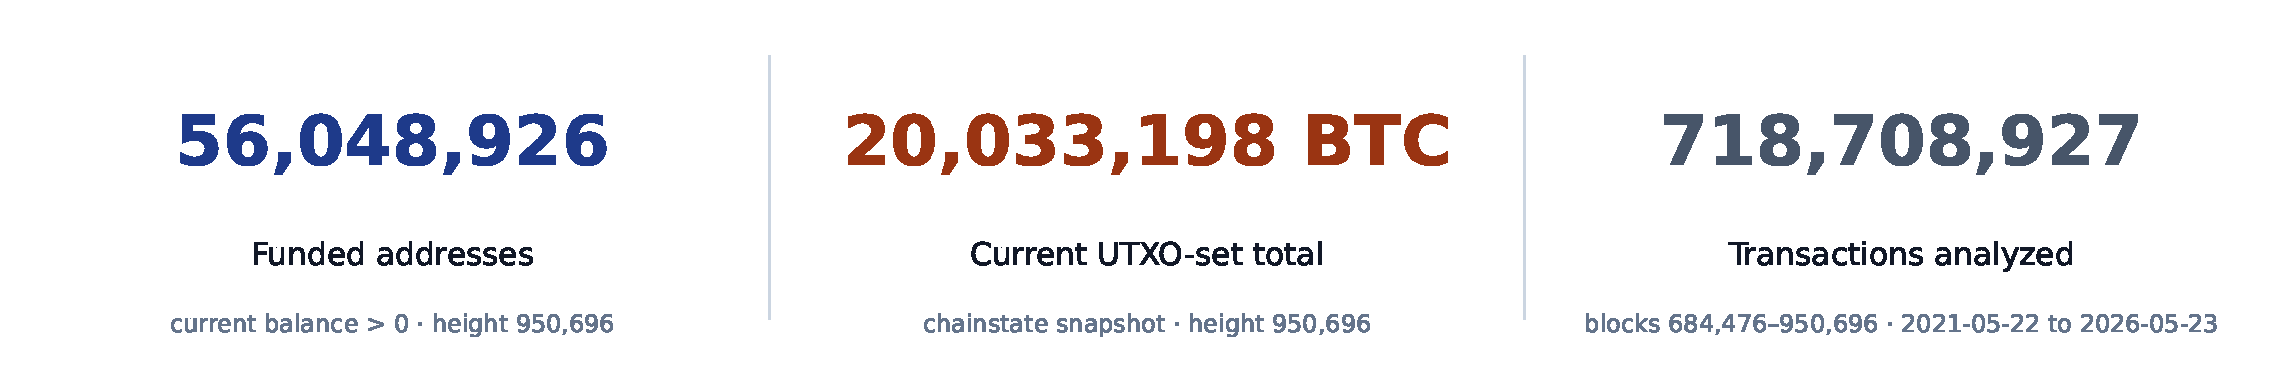
\includegraphics[width=0.95\textwidth]{figures/fig00_dataset_scale.pdf}
  \caption{Dataset scale for funded addresses and UTXO-set BTC at height
  950{,}696, and non-coinbase transactions in the five-year window.}
  \label{fig:dataset-scale}
\end{figure*}

Together these data support three claims. Much of the current BTC stock is
old, on-chain movement retains a large upper tail, and current address
balances are concentrated rather than diffuse.
The macro setting covers 2021 to 2026; the address-level evidence is a
full-node, current-output analysis.

\section{Measurement}\label{sec:design}

The empirical test uses four views of the same on-chain data. These are
current stock, transaction flow, dormancy cutoffs, and address balances.
The first three address the main functional question. The address view checks whether
the result is driven only by aggregate UTXO age.

The units of analysis are important. A UTXO is an unspent transaction
output, meaning one spendable coin fragment created by a past transaction. BTC
balance is value, measured by summing BTC amounts in UTXOs. UTXO count is
not value; it is the number of unspent outputs. An address can therefore
have a high BTC balance with one large UTXO, or a high UTXO count with many
tiny UTXOs. BTC share reports a share of value, while UTXO-count share
reports a share of output records. Address recency is the age of the newest
current UTXO assigned to that address.

Let $H$ be the chain tip height and let $\mathcal{U}_H$ be the UTXO set at
that tip. For output $u\in\mathcal{U}_H$, let $b_u$ be its BTC value,
$h_u$ its creation height, $s_u$ its output script family, and $a_u$ its
canonical address string when the parser can assign one. Stock and dormancy
use the same UTXO-age calculation. The stock view reports BTC by age
bucket; the dormancy view reports cumulative shares past fixed age cutoffs.
\begin{equation}
  S(\tau)=\frac{\sum_{u\in\mathcal{U}_H} b_u\,\mathbf{1}\{H-h_u\ge \tau\}}
                {\sum_{u\in\mathcal{U}_H} b_u},
\end{equation}
where $\tau$ is a block-age cutoff.

For the full-node flow window $\mathcal{B}$, let $x_t$ be the non-coinbase
BTC output sum of transaction $t$. The flow view estimates monthly
quantiles
\begin{equation}
  Q_{m,p}=\inf\left\{q: \frac{1}{|T_m|}\sum_{t\in T_m}
  \mathbf{1}\{x_t\le q\}\ge p\right\},
\end{equation}
where $T_m$ is the set of full-node-window non-coinbase transactions in
month $m$. These are output-sum quantiles before change-output correction.
They answer how large visible on-chain movements are during the block
window.

For address analysis, define the set of canonical addresses
$\mathcal{A}=\{a_u: a_u\neq \emptyset\}$. For address $a$, current balance
and current UTXO count are
\begin{equation}
  B_a=\sum_{u\in\mathcal{U}_H:a_u=a} b_u,\qquad
  C_a=\sum_{u\in\mathcal{U}_H:a_u=a} 1.
\end{equation}
These two address aggregates answer different questions. $B_a$ measures
how much BTC value is assigned to an address. $C_a$ measures how many
current output records are assigned to that address. Address dormancy uses
the most recent current UTXO at an address. This rule is conservative. If a
large old address receives one recent output, the whole address is
classified as recent. As a result, the old-address balance statistic is a
conservative summary of visibly unused address balances.

\section{Stock View: Current BTC by UTXO Age}\label{sec:stock}

We first measure the age distribution of current BTC. A UTXO is an unspent
transaction output, meaning a coin fragment created by an earlier transaction
and not yet spent by a later one. The UTXO set is therefore the live inventory
of spendable BTC at a given chain tip. Bitcoin Core's
\texttt{dumptxoutset} RPC writes that inventory to a file and reports the
snapshot base height and hash \cite{bitcoincore2026dumptxoutset}. The
snapshot used here is recorded at height 950{,}696.

The parser read 165.35 million UTXOs from that snapshot, totaling
20.03 million BTC. For each output, the parser kept the BTC amount and the
height $h$ of the transaction that created it. Age is computed by comparing
that creation height with the snapshot height as $(950{,}696-h)/144$ days.
We then place each output into an age bucket and sum BTC within that bucket. An
old UTXO therefore means that the output has not moved on chain since its
creating transaction.

The BTC-weighted buckets are large. At the snapshot date, 12.13 million BTC,
or 60.5\% of the UTXO set total, is at least one year old. Coins at least
three years old account for 8.61 million BTC, or 43.0\%; coins at least five
years old account for 6.68 million BTC, or 33.3\%. Figure~\ref{fig:stock-lens}
shows the distribution. This pattern is difficult to reconcile with
daily-payment use as the dominant on-chain pattern because much of the current
stock has not moved for years.

The limitation is motive and ownership. UTXO age is not the same as an
economic holding period. A coin can change hands inside a custodian or
through a legal claim without moving on chain, and a vault rotation can make
a long-term holder appear young. We therefore interpret the bucket totals as
a stock measure, namely the share of current BTC that has remained unspent
long enough to be consistent with savings balances.

\begin{figure}[!tbp]
  \centering
  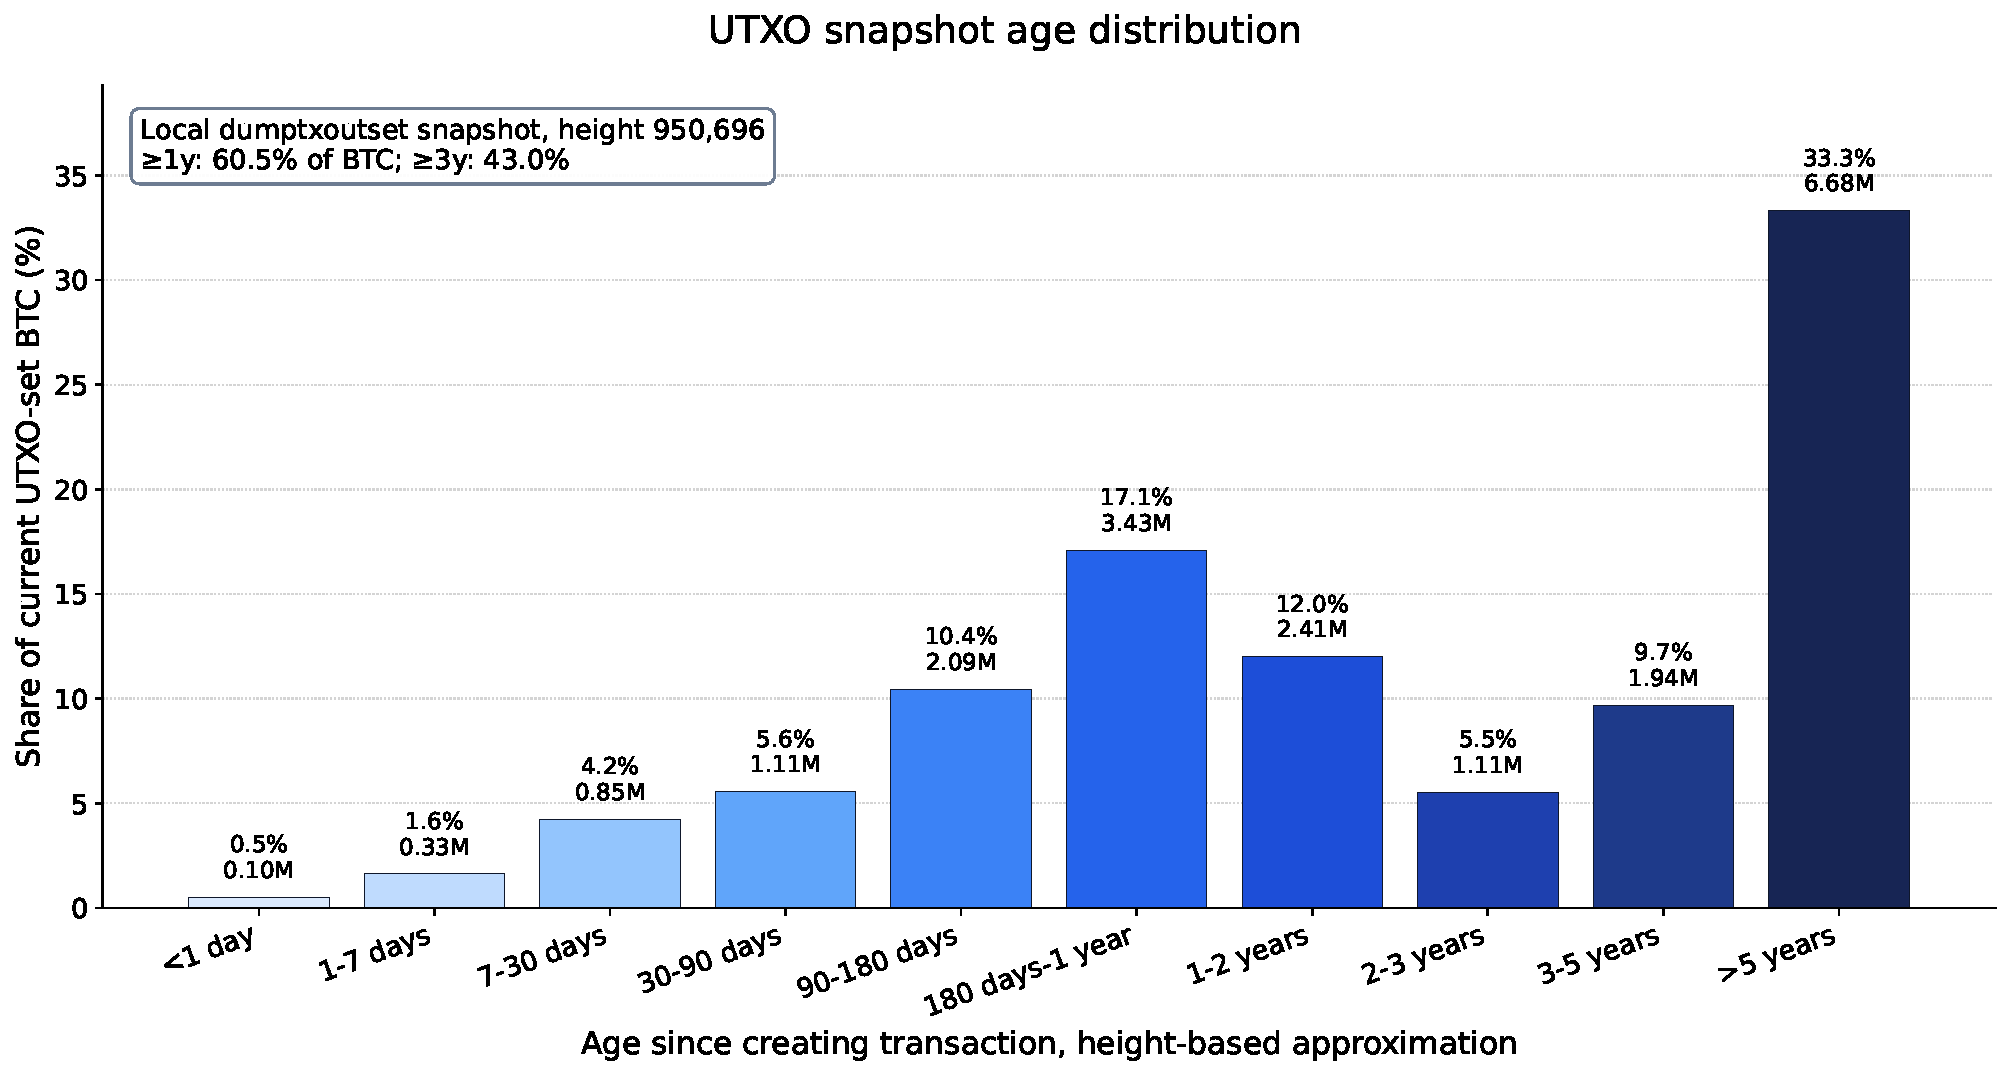
\includegraphics[width=0.95\linewidth]{figures/fig02_stock_lens.pdf}
  \caption{Bitcoin Core UTXO snapshot age distribution at height 950{,}696.}
  \label{fig:stock-lens}
\end{figure}

\section{Flow View: How Large On-Chain Transactions Are}\label{sec:flow}

The flow analysis measures the size of on-chain transactions when coins
move. This view studies activity rather than the full current UTXO stock.
The sample is all non-coinbase transactions in blocks 684{,}476 through
950{,}696. The script retrieves each block with Bitcoin Core RPC, drops the
coinbase transaction, and sums the BTC outputs of every other transaction.
It then groups transactions by month and records the median, p90, and p99
output sums. Figure~\ref{fig:flow-lens} puts time on the x axis and
transaction output sum on the y axis.

The full-node window covers about five years of block history. The median
transaction becomes smaller in BTC terms, but the upper tail remains large.
The yearly median falls from 0.0168~BTC in 2021 to 0.000750~BTC in 2026,
and the p90 falls from 1.50~BTC to 0.0944~BTC. Yet the p99 remains in
multi-BTC territory, with the full window's p99 about 26.61~BTC.
Table~\ref{tab:flow-summary} gives the full-node window values used to
interpret Figure~\ref{fig:flow-lens}. In Table~\ref{tab:flow-summary},
the rows are time slices. The first row is the full block
window from 2021 to 2026. The middle rows split the window by calendar
year, and the final row reports the end month. The columns report non-coinbase
transaction count and output-sum quantiles. Median is the typical
transaction, while p90 and p99 show the upper tail.

\begin{table}[!tbp]
  \centering
  \scriptsize
  \setlength{\tabcolsep}{2.5pt}
  \renewcommand{\arraystretch}{1.00}
  \begin{tabular}{@{}lrrrr@{}}
    \toprule
    \textbf{Slice} & \textbf{Tx M} & \textbf{Med. BTC} & \textbf{p90 BTC} & \textbf{p99 BTC} \\
    \midrule
    Full window & 718.7 & 0.00266 & 0.422 & 26.61 \\
    2021 & 55.4 & 0.0168 & 1.50 & 59.57 \\
    2022 & 93.1 & 0.0188 & 1.68 & 94.41 \\
    2023 & 153.4 & 0.00266 & 0.422 & 23.71 \\
    2024 & 192.2 & 0.00119 & 0.106 & 10.59 \\
    2025 & 153.7 & 0.00150 & 0.211 & 18.84 \\
    2026 & 71.0 & 0.000750 & 0.0944 & 16.79 \\
    May 2026 & 14.3 & 0.000422 & 0.0422 & 9.44 \\
    \bottomrule
  \end{tabular}
  \vspace{1em}
  \caption{Full-node-window non-coinbase transaction counts and output-sum
  quantiles. Tx M is millions of transactions; median, p90, and p99 are BTC
  output-sum quantiles before change-output correction; 2021 and 2026 are
  partial years.}
  \label{tab:flow-summary}
\end{table}

This flow result complements the stock result. Ordinary retail-sized
movement is smaller in BTC terms, but large balances still move through
settlement-sized transfers, batches, or treasury movements rather than small
daily purchases. The limitation is granularity. A large output sum can be a
settlement transfer, a batch payout, a wallet sweep, or a vault rotation.
Some Ordinals and BRC-20 activity also consumes blockspace without being a
payment \cite{rodarmor2023ordinals, domo2023brc20}. For that reason, this
measure is stated only as BTC output-sum size.

\begin{figure}[!tbp]
  \centering
  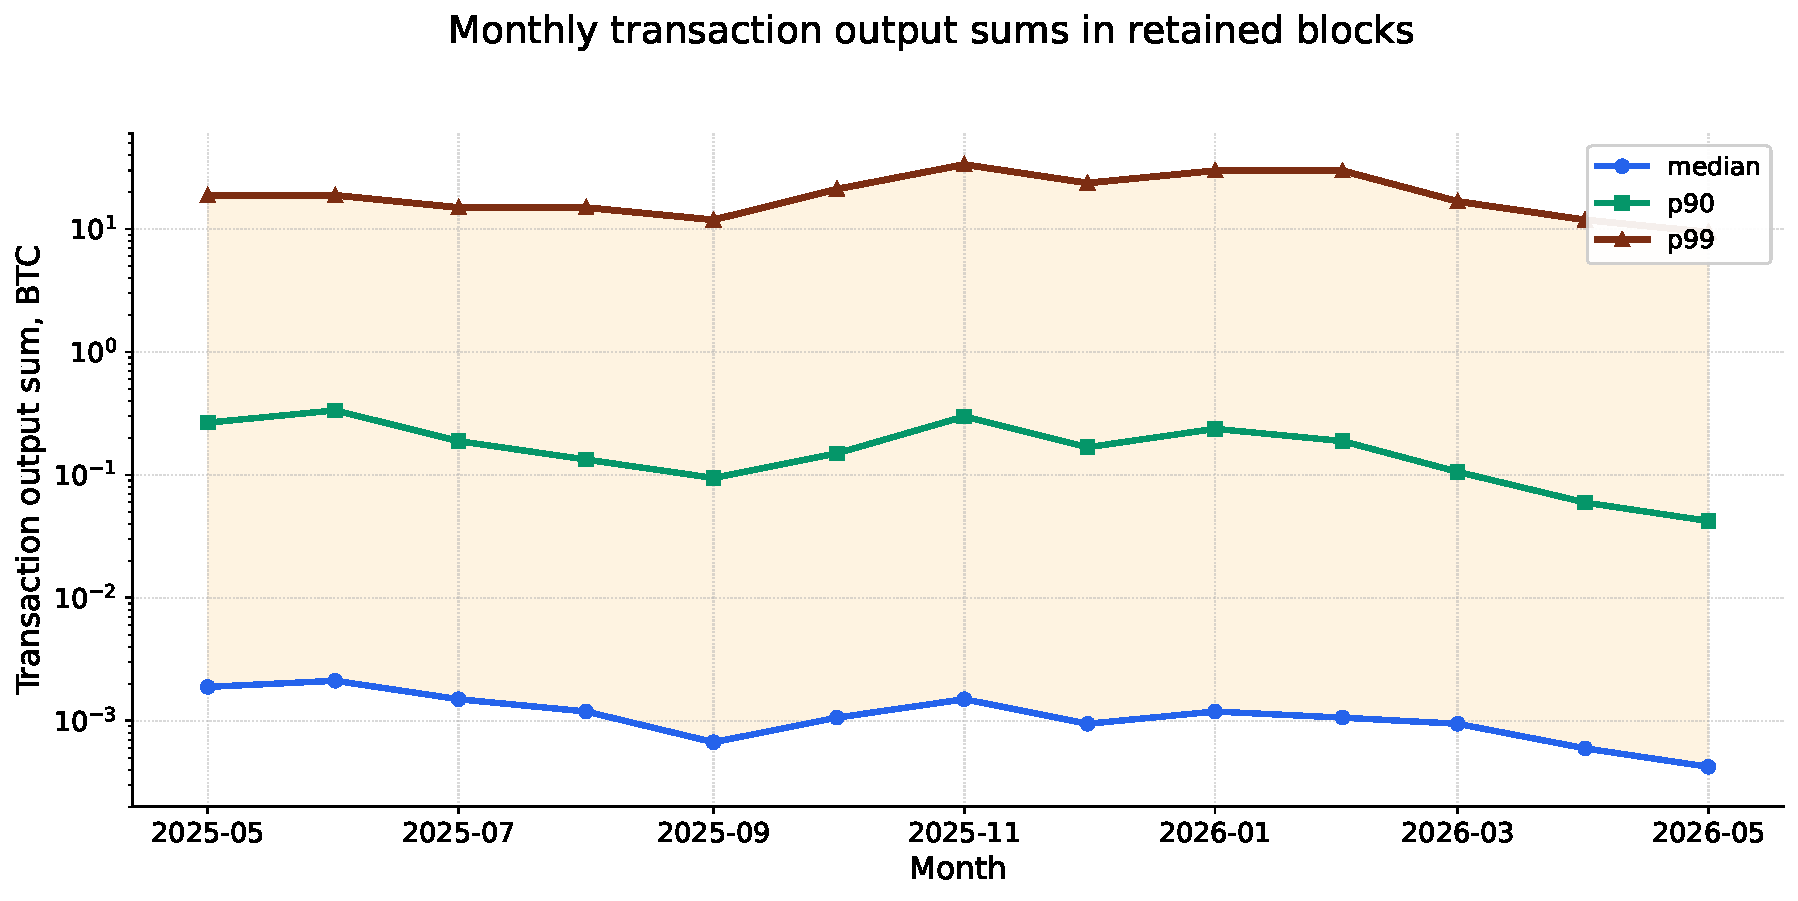
\includegraphics[width=0.95\linewidth]{figures/fig03_flow_lens_kde.pdf}
  \caption{Monthly full-node block transaction output sums in BTC units.}
  \label{fig:flow-lens}
\end{figure}

\section{Dormancy View: BTC Still Unspent After Time Cutoffs}\label{sec:sink}

The dormancy view uses the same UTXO-age method as the stock view, but
reports cumulative cutoffs instead of buckets. It reports the share of
current BTC that remains unspent after one day, one week, one month, three
months, six months, one year, two years, three years, or five years.

The cumulative pattern reinforces the stock view. At height 950{,}696,
77.6\% of BTC is at least 180 days old, 60.5\% is at least one year old,
48.5\% is at least two years old, 43.0\% is at least three years old, and
33.3\% is at least five years old. Figure~\ref{fig:sink-lens} plots these
thresholds directly. This does not imply that every old output is deliberate
cold storage. It shows that a large current stock has remained unspent far
longer than a daily payment balance normally would.

The limitation is motive. Lost keys, omnibus custody, legal restriction,
deliberate vaulting, and ordinary long-term saving can look identical in a
UTXO snapshot. The evidence here is therefore an age measure, not a claim
about why any particular coin remained unspent.

\begin{figure}[!tbp]
  \centering
  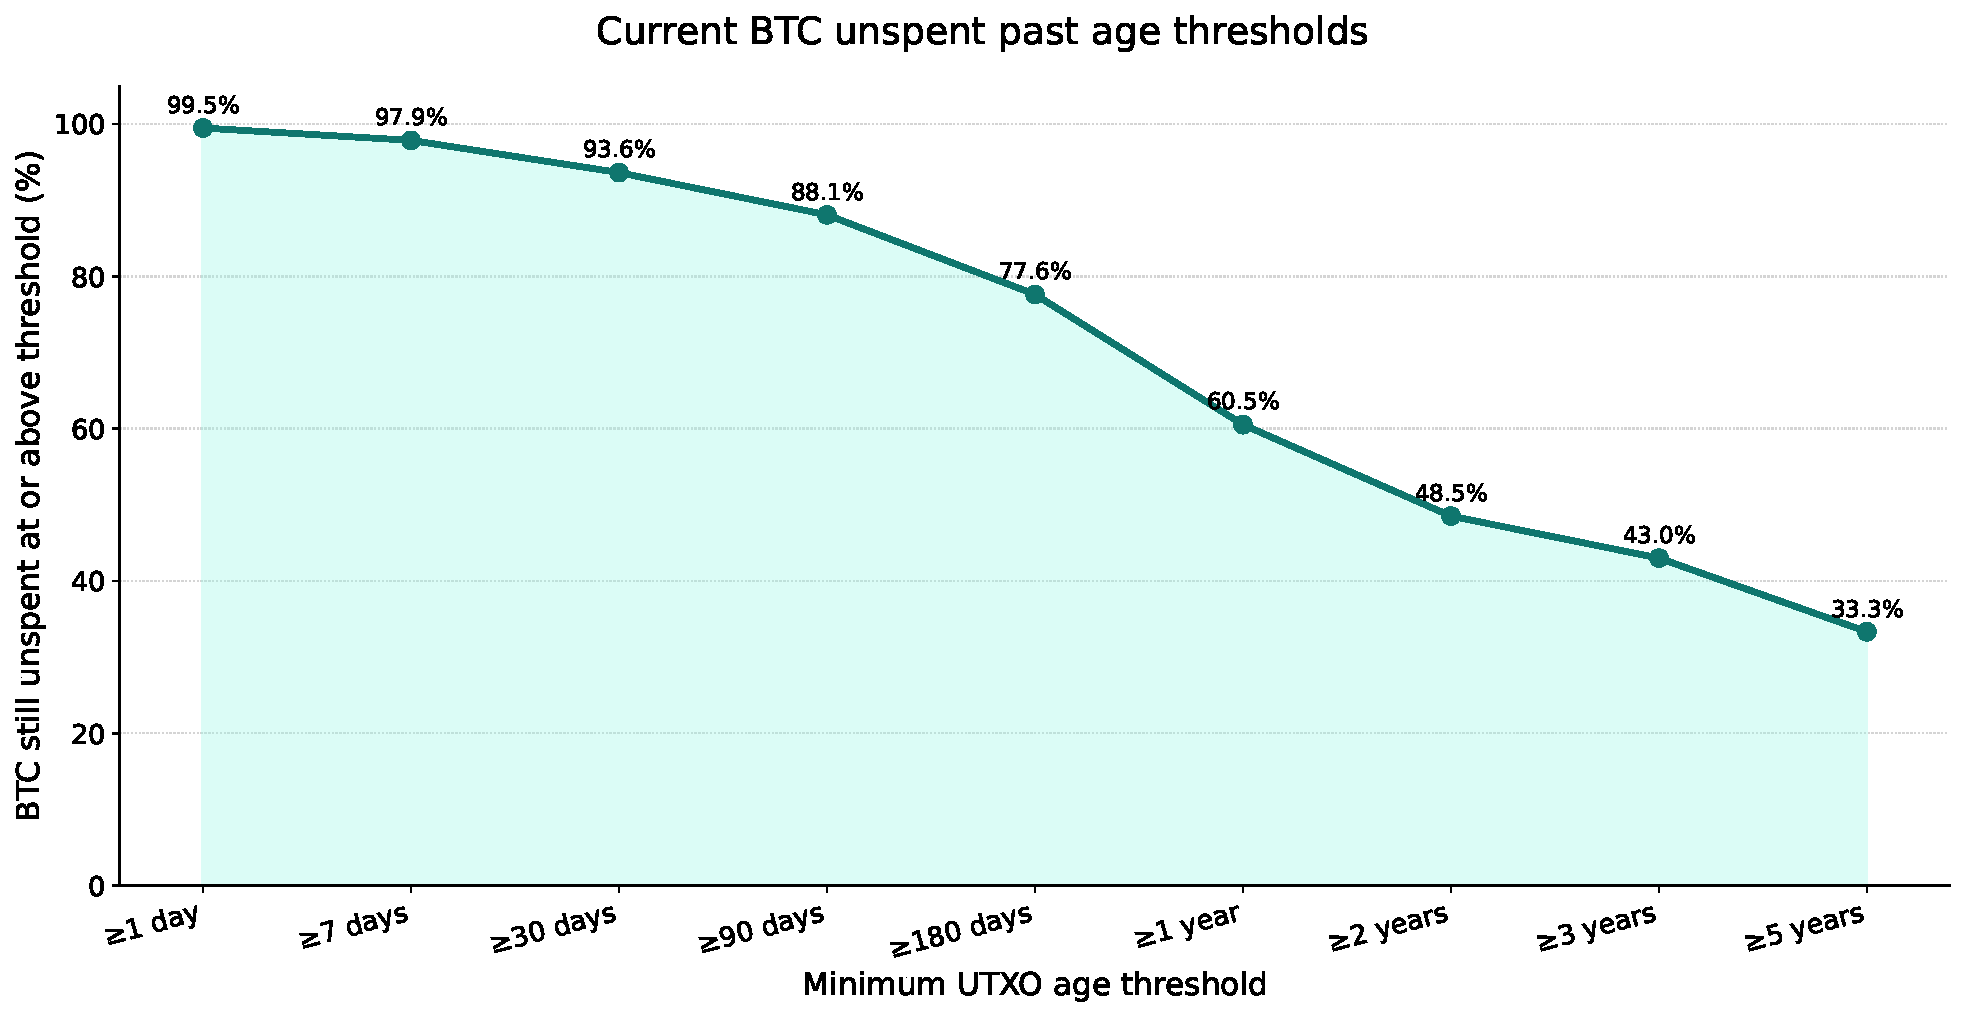
\includegraphics[width=0.95\linewidth]{figures/fig04_sink_lens.pdf}
  \caption{BTC still unspent past age thresholds in the chainstate snapshot.}
  \label{fig:sink-lens}
\end{figure}


\section{Address-Level Evidence from Transaction Data}\label{sec:address-level}

This section asks whether the transaction data resemble a retail payment
network after current UTXOs are grouped by address. The address data do not
show that pattern. They are concentrated. A small set of recent addresses
holds most address-attributable BTC, many old addresses hold smaller
balances, and another set of addresses manages very large numbers of small
UTXOs.

The measurement is direct. Each current UTXO has a value, creation height,
script family, and, when possible, a canonical address string. Grouping
current UTXOs by address gives four observable facts. These are how much BTC an
address holds, how many current UTXOs it holds, which script family those
outputs use, and how recent the newest current UTXO at that address is. The
analysis does not identify owners or label exchanges. It only describes the
current address distribution.


The receiver-side address pass adds a transaction-flow check. Over the
full-node block window, the Bitcoin Core block walk covers 266,221 blocks
and assigns 1,836,694,788 address-attributable output records, totaling
2,941,289,223.11 BTC, to canonical address strings. This result does not
label owners. It shows that the transaction data behind the current-balance
address table also contain a large recent receiver-side address set.

\subsection{Coverage and script types}

In Figure~\ref{fig:script-family-mix}, UTXO-count share and
BTC-balance share are compared by script family. In
Figure~\ref{fig:script-value-per-utxo}, the same script families are
shown by average BTC per current UTXO.

The parser assigns canonical addresses to 19.92 million BTC, or 99.4\% of
the snapshot balance, across 56.05 million addresses. The remaining
0.11 million BTC does not enter address-balance totals because those
outputs do not receive a canonical address string in this parse. The
address results therefore cover almost all of the live BTC stock. By output
count, the address parse covers 162.39 million of the snapshot's
165.35 million UTXO records; records without a canonical address string stay
outside it.

Script family shows how current BTC is distributed across output types. The
categories used here are p2pk, p2pkh, p2sh, p2wpkh, p2wsh, p2tr, multisig,
and other. Native SegWit pay-to-witness-public-key-hash holds 8.11 million
BTC, legacy pay-to-public-key-hash holds 5.93 million BTC,
pay-to-script-hash holds 3.94 million BTC, and native SegWit script-hash
holds 1.33 million BTC. Together those mature families hold about
19.31 million BTC. P2TR, the Pay-to-Taproot family introduced by Taproot,
has a different profile. It has 54.35 million current UTXOs, or 33.5\% of current UTXO
rows, but only 197{,}376 BTC, or 1.0\% of current BTC.
Pay-to-public-key is the opposite case, with few current outputs but
0.41 million BTC. Figure~\ref{fig:script-family-mix} shows this split for
the six families with current rows (multisig and other have none in this
parse), and Figure~\ref{fig:script-value-per-utxo} shows the corresponding
BTC-per-UTXO scale.

Each script family is interpreted along two dimensions. UTXO share measures
how many current output records use that script family. BTC share measures
how much value those records carry. Native SegWit p2wpkh is large on both
axes, with 29.9\% of current UTXOs and 40.7\% of current BTC. Legacy
p2pkh has 27.4\% of current UTXOs and 29.8\% of current BTC. P2SH has
a smaller output share, 7.5\%, but a larger value share, 19.8\%. P2WSH is smaller still by output
count, 1.7\%, but holds 6.7\% of current BTC. These mature families hold
most of the visible BTC stock.

P2TR is the count-heavy case. It has the largest current UTXO count in this
snapshot, but the BTC held in those outputs is small. This means Taproot
matters for current output formation and script adoption, but it is not the
script family holding most spendable BTC. P2PK is the reverse legacy case.
It has very few outputs but a large balance share. The script-family results
therefore support the paper's main distinction. Output count describes
activity and record structure, while BTC balance describes stored value.

Taproot timing is reported as a P2TR-specific check, not as another script
family category. The daily counts come from a retained third-party adoption
snapshot and provide context rather than a local-node measurement. Taproot
activated on 2021-11-14. The same-day protocol rows record 208 P2TR
outputs and 75 transactions spending P2TR outputs. By
2026-05-24, the daily counts are 108{,}503 P2TR outputs and 45{,}864
transactions spending P2TR outputs. Taproot therefore has visible transaction
use, but the current BTC balance remains small relative to mature script
families.

Bitcoin clearly has new script forms. The question for this paper is
whether those script forms change where stored BTC is held. The answer from
the current output set is limited but direct. P2TR is large by output count
and small by BTC balance.
P2WPKH, P2PKH, P2SH, and P2WSH are the large balance families. P2PK is a
legacy balance pocket with very little current output formation. The script
mix therefore separates new transaction formats from the main locations of
stored BTC.

\begin{figure*}[!tbp]
  \centering
  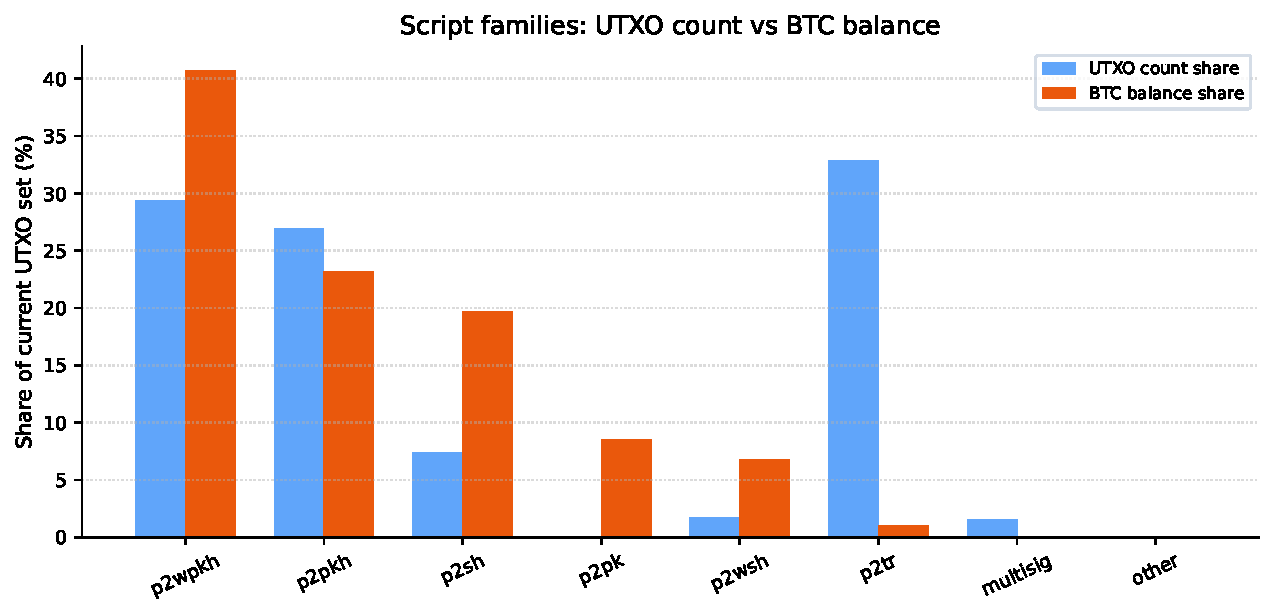
\includegraphics[width=0.78\textwidth]{figures/fig05_script_family_mix.pdf}
  \caption{Script families separate output count from stored BTC value.}
  \label{fig:script-family-mix}
\end{figure*}

\begin{figure*}[!tbp]
  \centering
  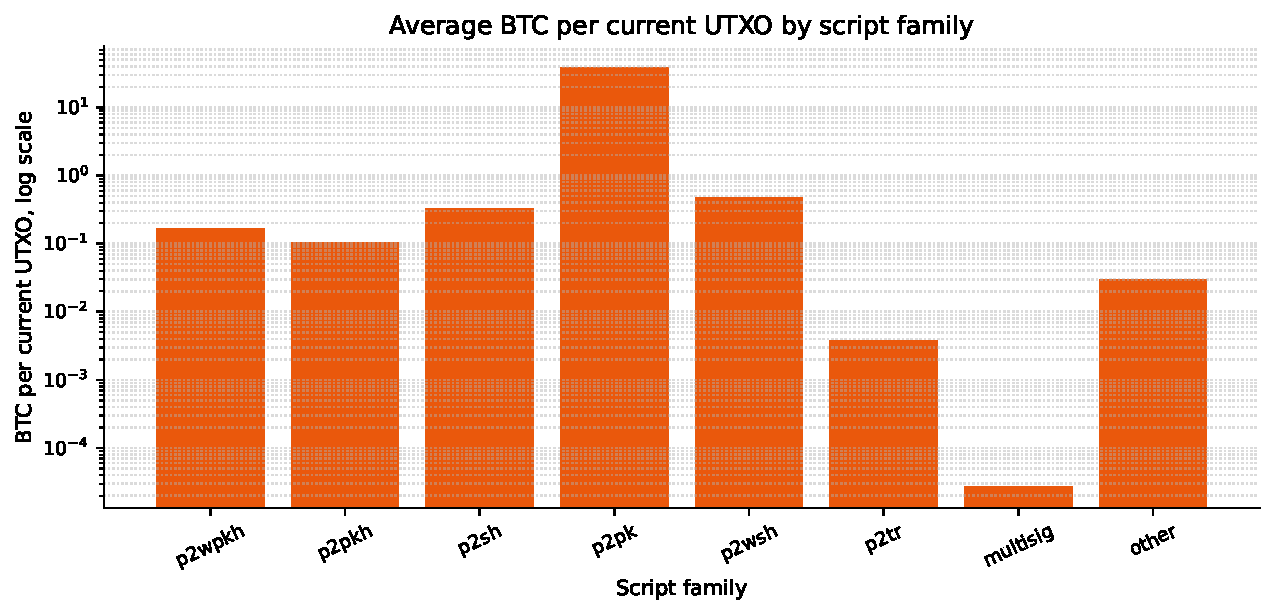
\includegraphics[width=0.78\textwidth]{figures/fig06_script_value_per_utxo.pdf}
  \caption{Average BTC per current UTXO differs sharply across script families.}
  \label{fig:script-value-per-utxo}
\end{figure*}

\subsection{Address recency}

In Figure~\ref{fig:address-one-year}, address share and BTC share are
compared for addresses whose newest current UTXO is less than five years old
versus at least five years old. In Table~\ref{tab:address-numeric}, the
recency rows give the exact address counts, BTC totals, and percentages.

Address recency is based on the newest current UTXO at each address. If an
address contains one ten-year-old UTXO and one recent UTXO, the address
is classified as under five years old. This rule is conservative for
old-address claims, because one new output can move the whole address into
the recent category.

Under that rule, 34.28 million addresses have a newest current UTXO less
than five years old. They are 61.2\% of all addresses and hold
18.27 million BTC, or 91.7\% of address-attributable BTC. Addresses with no
current UTXO younger than five years number 21.76 million, or 38.8\% of
addresses, but hold only 1.65 million BTC, or 8.3\% of
address-attributable BTC. The recency block in Table~\ref{tab:address-numeric}
shows the two-row partition; the two rows add to 100\% within that block.
Figure~\ref{fig:address-one-year} plots the same asymmetry.

The central point is the gap between address count and BTC share. More than
a third of funded addresses have been untouched for at least five years, yet
they hold only 8.3\% of address-attributable BTC. Nearly all value is held at
addresses with at least one output formed inside the five-year window. This
does not make window-recent BTC a payment measure. It shows that large
balances can be held at addresses that also receive a current output within
the window. Recency is therefore useful alongside UTXO age. UTXO age
measures coin-fragment age, while address recency measures the newest output
at an address.

This address result does not contradict the stock and dormancy results. An
address can be classified as recent because one current output is recent,
while other outputs at the same address are much older. The address measure
is therefore strict against old-address claims and useful for measuring
concentration. If most BTC were spread across ordinary payment addresses,
the recent-address share and the BTC share would be closer together.
Instead, value is much more concentrated than address count.

\subsection{UTXO frequency and balance concentration}

In Table~\ref{tab:address-numeric}, the UTXO-count block gives the
address and BTC shares for each count bucket. In
Figure~\ref{fig:address-count-rank}, the left panel shows the
address-count distribution across UTXO-count buckets and the right panel
ranks the top ten addresses by current BTC balance. In
Figure~\ref{fig:address-one-year}, panel B plots the same UTXO-count buckets
and panel C compares the two top-100 tails.

UTXO frequency measures how many current outputs are assigned to each
address. If the chain were mainly a retail payment network, value would be
spread broadly across many small balances. In the current data, addresses
with one UTXO are 85.3\% of addresses but hold 24.4\% of
address-attributable BTC. Addresses with more than ten current UTXOs are
about 2.3\% of addresses but hold 28.4\% of address-attributable BTC.
Addresses with more than one hundred UTXOs are 0.23\% of addresses and
hold 1.67 million BTC. The UTXO-count block in
Table~\ref{tab:address-numeric} is separate from the recency block; its rows
also add to 100\% within that block. Figure~\ref{fig:address-count-rank}
separates the issue into address count and balance rank.

\begin{table*}[!tbp]
  \centering
  \scriptsize
  \setlength{\tabcolsep}{5pt}
  \renewcommand{\arraystretch}{1.08}
  \begin{tabular}{@{}llrrrr@{}}
    \toprule
    \textbf{Block} & \textbf{Category} & \textbf{Addresses} & \textbf{Address \%} & \textbf{BTC} & \textbf{BTC \%} \\
    \midrule
    Denominator & All address-attributable & 56{,}048{,}926 & 100.00 & 19{,}920{,}500 & 100.00 \\
    \midrule
    Recency & Newest current UTXO $<$5 yr & 34{,}284{,}347 & 61.17 & 18{,}266{,}630 & 91.70 \\
    Recency & Newest current UTXO $\ge$5 yr & 21{,}764{,}579 & 38.83 & 1{,}653{,}871 & 8.30 \\
    \midrule
    UTXO count & 1 UTXO & 47{,}808{,}232 & 85.30 & 4{,}868{,}115 & 24.44 \\
    UTXO count & 2 UTXOs & 3{,}496{,}008 & 6.24 & 2{,}756{,}193 & 13.84 \\
    UTXO count & 3 to 5 UTXOs & 2{,}458{,}366 & 4.39 & 4{,}878{,}748 & 24.49 \\
    UTXO count & 6 to 10 UTXOs & 989{,}652 & 1.77 & 1{,}757{,}094 & 8.82 \\
    UTXO count & 11 to 100 UTXOs & 1{,}168{,}758 & 2.09 & 3{,}992{,}500 & 20.04 \\
    UTXO count & $>$100 UTXOs & 127{,}910 & 0.23 & 1{,}667{,}851 & 8.37 \\
    \bottomrule
  \end{tabular}
  \vspace{1em}
  \caption{Current address-attributable BTC split by recency and UTXO count.}
  \label{tab:address-numeric}
\end{table*}

The top-100 comparisons separate balance concentration from output-count
concentration. The top 100 addresses by current BTC balance hold
3.02 million BTC, or 15.1\% of address-attributable BTC. The top 100
addresses by UTXO count carry 8.80 million current UTXOs, or 5.4\% of all
UTXOs, but only about 1{,}466 BTC. Figure~\ref{fig:address-one-year} panel C
puts those two top-100 measurements on the same scale. The largest
BTC-balance addresses show where current value is concentrated. The largest
UTXO-count addresses show where many output records are being managed.

The count side and the value side therefore describe different uses.
Count-heavy addresses can come from repeated receipts, payout systems, dust,
consolidation, or other output-management workflows. Balance-heavy addresses
show where current BTC value is concentrated. A daily retail payment network
would not require this sharp split; custody, settlement, and
output-management workflows naturally can produce it.

\begin{figure*}[!tbp]
  \centering
  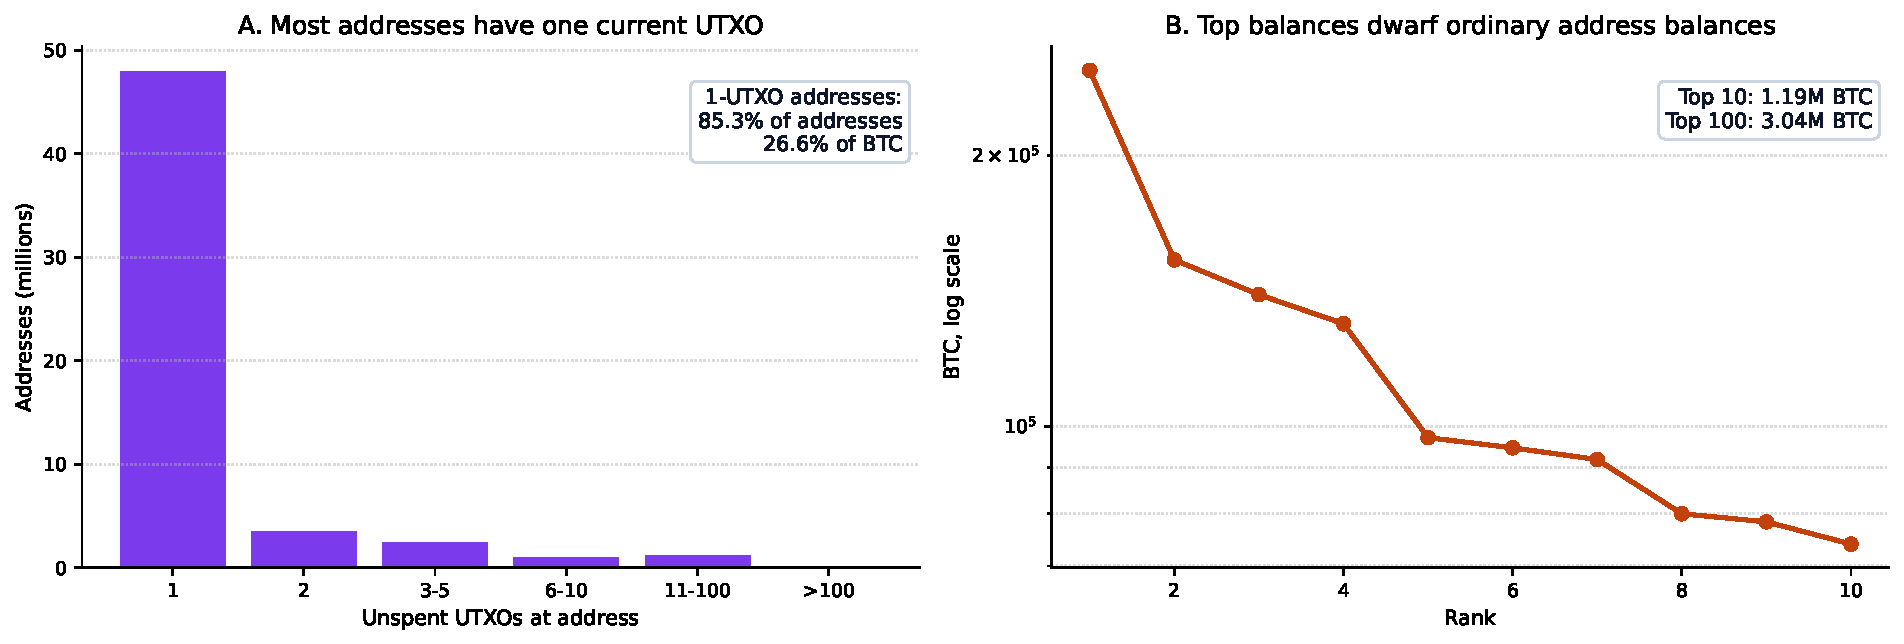
\includegraphics[width=0.95\textwidth]{figures/fig05_address_count_rank.pdf}
  \caption{Address count is dominated by one-UTXO addresses, while BTC value
  has a separate high-balance tail.}
  \label{fig:address-count-rank}
\end{figure*}

\begin{figure*}[!tbp]
  \centering
  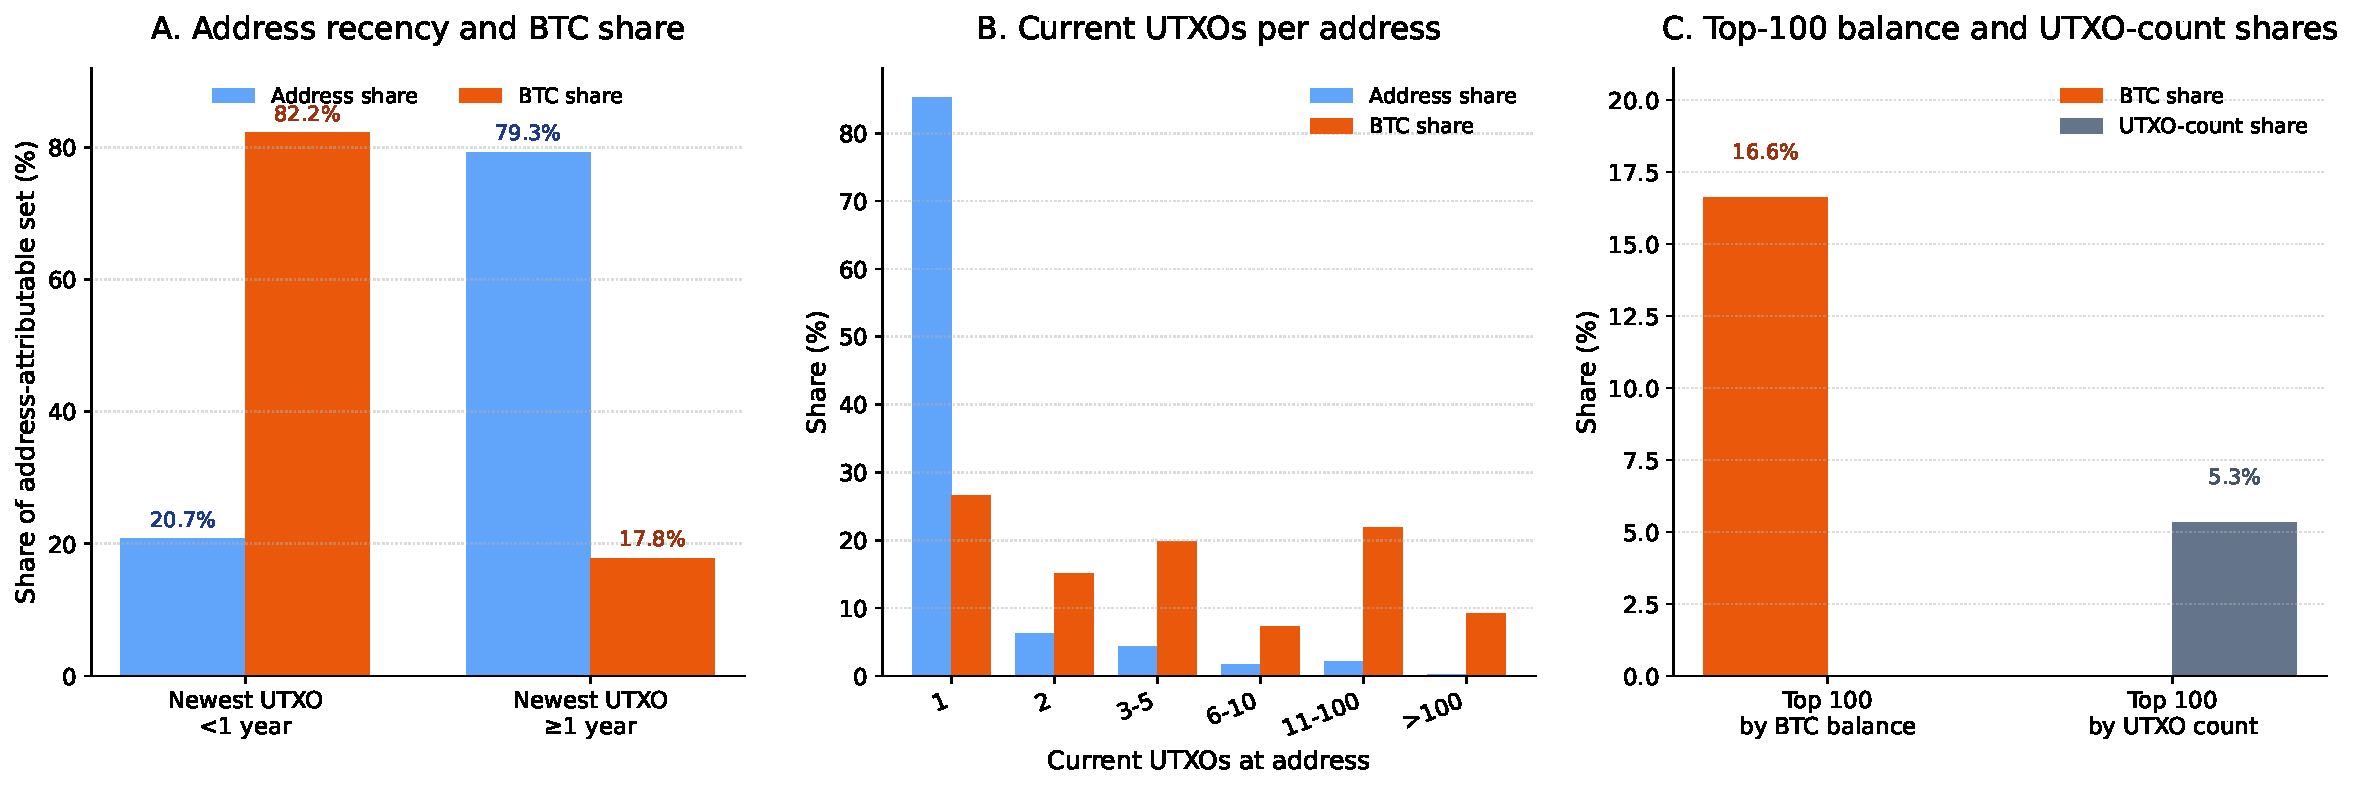
\includegraphics[width=0.95\textwidth]{figures/fig06_address_one_year.pdf}
  \caption{Address recency, UTXO-count buckets, and top-100 concentration
  for the current address-attributable set.}
  \label{fig:address-one-year}
\end{figure*}



\section{How the Evidence Fits Together}\label{sec:convergence}

The measurements support the same interpretation from different angles. The
stock view shows that 60.5\% of current BTC is at least one year old and
43.0\% is at least three years old. The address results show that the same
current stock is not distributed evenly across addresses. The top 100
balance addresses hold 3.02 million BTC, and mature script families hold
about 19.31 million BTC. UTXO age and address concentration are different
measurements, but both are consistent with stored value rather than broad
retail working balances.

The dormancy cutoffs and address recency also fit together. The dormancy
view shows that 33.3\% of BTC has remained unspent for at least five years.
Address recency shows that the 38.8\% of addresses untouched for at least
five years hold only 8.3\% of address-attributable BTC, while addresses with
a newer current output hold 91.7\%. Large balances can therefore be held at
addresses that occasionally receive new outputs. Recent address activity does
not overturn the old-coin result.

The flow view and UTXO-count buckets explain another part of the pattern.
The full-node transaction distribution has a small center and a large p99
tail. At the same time, addresses with more than ten current UTXOs are only
about 2.3\% of addresses but hold 28.4\% of address-attributable BTC, while
the top 100 UTXO-count addresses contain 8.80 million current UTXOs and only
about 1{,}466 BTC. This pattern is consistent with batching, consolidation,
custody operations, and large transfers. It is less consistent with a
network dominated by small daily payments.

The script-family results add a final check. Taproot is visible in output
and spend activity, but P2TR holds only about 1.0\% of current BTC. Mature
script families hold most BTC, while newer output forms are more visible in
count than in stored value. Protocol adoption changes the form of some
transactions, but it does not change where most current BTC is held.

The conclusion does not depend on a single statistic. If only UTXO age were
old, lost coins or vaulting could explain much of the result. If only
transaction p99 were large, batching could explain much of the result. If
only top addresses were large, exchange custody could explain much of the
result. In this case, the separate measurements align. They include old stock, BTC that
remains unspent well beyond daily-payment timeframes, large-transfer tails,
concentrated address balances, many-output operational addresses, and
mature-script value.

These measurements still do not identify motive for any particular coin or
address. UTXO age can overstate saving, flow size can mix settlement with
batching, and address balances can combine many users behind one script. The
claim is therefore about the aggregate shape of the data, not about any
single holder. That aggregate shape points away from an on-chain record
dominated by daily retail payments.

A daily retail payment network would be expected to leave different
patterns. Less BTC would remain unspent for years. The flow distribution
would depend less on a large-transfer upper tail. Address recency would not
leave a large five-year-dormant address group holding almost no value.
UTXO-count rank and balance rank would be closer together. New payment forms
would dominate both output count and BTC value, not mainly output count. The
observed data do not match that profile.

This interpretation does not require Bitcoin to have only one use. Bitcoin
can still process on-chain payments, and some current outputs are small
payment, change, or wallet-management outputs. The claim is about the
dominant visible pattern in the on-chain data. Across the measurements, the
record is old, concentrated, uneven, layered by script family, and large at
the upper tail. That is the basis for reading the on-chain record from 2021 to 2026
as store-of-value and settlement infrastructure first, rather than as a
daily payment rail first.

\section{Limits and Validity}\label{sec:robustness}

The main validity check is unit separation. The stock and dormancy results
use the current chainstate snapshot. The flow results use full-node block
transaction output sums. The address results use canonical address strings
assigned by the parser. Because these are different measurements, the
conclusion does not rest on a single statistic.

There are five main limitations. First, age is not motive. A five-year UTXO
can be lost, legally transferred off chain, held in custody, or intentionally
saved. Lost coins and custodial cold storage are not separately measured
here, and both can raise the old-stock share. The stock and dormancy claims
are therefore stated as on-chain immobility, not as intent. Second,
transaction output sums are not exact payment amounts. They include change,
batching, vault rotations, and service sweeps. The flow result is therefore
an on-chain movement-size measure, not a consumer-payment classifier. Third,
addresses are not wallets. Modern wallets rotate addresses, while custodians
and services can aggregate many users behind one address or script policy.
Fourth, address recency is based on the newest current UTXO at each address,
so one new output can make an otherwise old address appear recent. Fifth,
on-chain transaction data do not observe Lightning channels,
custodial-internal transfers, or sidechain activity. If payment activity
moves to those venues, the Bitcoin blockchain can appear less payment-like
even if total Bitcoin payment use does not fall.

These limitations do not change the main conclusion because the paper does
not label any single transaction or address. It describes the distribution
of the on-chain data. A payment-dominated on-chain system would be expected
to have a smaller old-stock share, a less settlement-heavy upper tail, and a
less concentrated current address structure. The measurements show the
opposite. The most defensible interpretation is therefore that the measured
on-chain data are more consistent with savings, custody, and settlement
infrastructure than with a daily payment rail. Within the 2021 to 2026 window
itself, only the flow view is measured across time; the stock, dormancy, and
address views describe the end state at height 950{,}696 and are read as
consistent with the shift, not as a full time series of it.

\section{Conclusion}\label{sec:verdict}

The evidence supports a clear conclusion. \btc{}'s on-chain transaction data
are more consistent with store-of-value and settlement use than with daily
payment use. The stock view shows that 60.5\% of current BTC is at least one
year old and 43.0\% is at least three years old. The dormancy view shows
that 33.3\% remains unspent after at least five years. The full-node flow
view shows a transaction distribution from 2021 to 2026 with a small center
and a large-transfer upper tail. The address view shows that 19.92 million BTC
maps to 56.05 million canonical addresses and that value is concentrated
rather than spread across daily-use balances. The top 100 balance addresses
alone hold 15.1\% of address-attributable BTC, while the 38.8\% of addresses
untouched for at least five years hold only 8.3\%.

The claim is intentionally limited. It does not say that every holder is
saving, every large transaction is settlement, or every address is a custody
address. It says that the measured Bitcoin transaction data reject the
simplest daily-payment interpretation. Bitcoin still supports on-chain
payments, but the observed transaction data are more consistent with
savings, custody, large transfers, and operational consolidation.


\appendices

\section{Data Sources and Reproducibility}\label{app:data}

The reproducibility repository is \url{https://github.com/xodn348/ray.project-reproducibility}.
Table~\ref{tab:repro-sources} lists the source tables and scripts used for
each reproduced figure and summary table. The full-node flow artifact is
\datafile{data/phase2/rpc_retained_flow_fullnode_20260529T193328Z};
the address summaries are rebuilt from
\datafile{data/phase2/address_core_stage1}. The underlying address
database and receiver-side shard files are local-only artifacts and are
not redistributed; the committed summaries are the reproducible
interface. The rebuild entry point is
\datafile{scripts/phase2/regen_all.sh}; it regenerates the figures and
rebuilds the IEEE PDF.

\begin{table*}[!tbp]
  \centering
  \scriptsize
  \setlength{\tabcolsep}{3.5pt}
  \renewcommand{\arraystretch}{1.08}
  \begin{tabular}{@{}L{0.16\textwidth}L{0.25\textwidth}L{0.27\textwidth}L{0.22\textwidth}@{}}
    \toprule
    \textbf{Output} & \textbf{Measurement} & \textbf{Data} & \textbf{Script} \\
    \midrule
    Figure~1 & Macro/protocol timing & Hand-curated event arrays in the script; source records in \datafile{data/events/timeline.csv}; \datafile{data/events/regulatory_events.csv} & \datafile{scripts/figures/fig01_macro_protocol_timeline.py} \\
    Figure~2 & Dataset scale (addresses, UTXO-set BTC, transactions) & \datafile{data/phase2/address_core_stage1/coverage_summary.json}; \datafile{data/phase2/utxo_snapshot_20260523/utxo_age_buckets.csv}; \datafile{rpc_retained_flow_blocks.csv} & \datafile{scripts/figures/fig00_dataset_scale.py} \\
    Figures~3 and~5 & Current UTXO stock and dormancy age & \datafile{data/phase2/utxo_snapshot_20260523/manifest.json}; \datafile{utxo_age_buckets.csv}; \datafile{utxo_cumulative_age.csv} & \datafile{scripts/figures/fig02_phase2.py}; \datafile{fig04_phase2.py} \\
    Table~I and Figure~4 & Full-node block transaction output sums & \datafile{data/phase2/rpc_retained_flow_fullnode_20260529T193328Z/manifest.json}; \datafile{rpc_retained_flow_summary.csv}; \datafile{rpc_retained_flow_blocks.csv}; \datafile{rpc_retained_flow_histogram.csv} & \datafile{scripts/figures/fig03_phase2.py} \\
    Figures~6 and~7 & Script-family UTXO count, BTC balance, and BTC per UTXO & \datafile{data/phase2/address_core_stage1/coverage_summary.json}; \datafile{script_type_balance.csv} & \datafile{scripts/figures/fig05_address_level.py} \\
    Table~II and Figures~8 and 9 & Address recency, UTXO-count buckets, and top-rank tails & \datafile{data/phase2/address_core_stage1/dormancy_balance.csv}; \datafile{utxo_count_distribution.csv}; \datafile{top_balance.csv}; \datafile{top_utxo_count.csv}; \datafile{coverage_summary.json} & \datafile{scripts/figures/fig05_address_level.py}; \datafile{fig06_address_one_year.py} \\
    \bottomrule
  \end{tabular}
  \vspace{1em}
  \caption{Data tables and scripts used to reproduce the paper measurements and figures.}
  \label{tab:repro-sources}
\end{table*}


\bibliographystyle{IEEEtran}
\bibliography{\paperbibfile}

\end{document}
